
\frame
{
\frametitle{Representación Matemática}
\framesubtitle{Parámetros}
    \begin{itemize}
        \item \blue{$cN$}: Número total de autos.
        \item \blue{$oN$}: Número total de opciones disponibles.
        \item \blue{$tN$}: Número total de tipos/clases de autos.
    \end{itemize}
}

\frame
{
\frametitle{Representación Matemática}
\framesubtitle{Variables}
    \begin{itemize}
        \item \blue{$nMax_{ij}$}: Número máximo de autos con la opción $i$ en una subsecuencia $j$.
        \item \blue{$n_{ij}$}: Número de autos con la opción $i$ en una subsecuencia $j$.
        \item \blue{$sMax_{i}$}: Tamaño de la subsecuencia $j$ donde deben haber $nMax_{ij}$ autos.
        \item \blue{$q_{k}$}: Cantidad de autos del tipo/clase $k$.
        \item \blue{$types_{il}$}: Booleano que indica si la opción $i$ está presente en el auto $l$.
    \end{itemize}
}

\frame
{
\frametitle{Representación Matemática}
\framesubtitle{Función objetivo}

    $$FO\ :\ Min\ \sum\limits_{i=1}^{oN} \sum\limits_{l=1}^{cN} \sum\limits_{j=0}^{sMax_{i}} types_{il}\cdot (n_{ij} - nMax_{ij}), \forall n_{ij} > nM_{ij}$$
}

\frame
{
\frametitle{Representación Matemática}
\framesubtitle{Restricciones}

Restricciones Duras
    $$\sum\limits_{k=1}^{cN} q_{k} = cN$$

Restricciones Blandas
    $$\sum\limits_{i=1}^{oN} \sum\limits_{l=1}^{cN} \sum\limits_{j=0}^{sMax_{i}} types_{il}\cdot n_{ij} \leq nMax_{ij}$$
}

\frame
{
\frametitle{Representación EDD}
\begin{center}
	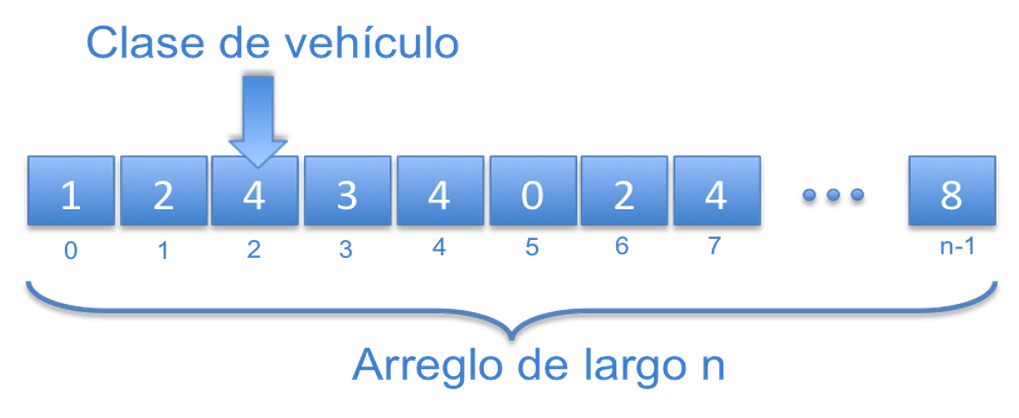
\includegraphics[width=0.8\textwidth]{img/representacion}
\end{center}
}


\frame
{
\frametitle{Representación EDD}
\framesubtitle{Individuos y Restricciones}
\begin{columns}
	\begin{column}{0.3\textwidth}
    $\textbf{struct}\ cell$:

        \begin{itemize}
            \item $\textbf{int}\ gene[VARS]$
            \item $\textbf{int}\ fitness$
            \item $\textbf{double}\ rfitness$
            \item $\textbf{double}\ cfitness$
        \end{itemize}
	\end{column}
	\begin{column}{0.7\textwidth}
		Número máximo de \blue{autos} por subsecuencia
		$$\textbf{int}\ numMaxCarOptSeq[N]$$
	
		Tamaño \blue{subsecuencia}
		$$\textbf{int}\ sizeMaxCarOptSeq[N]$$
	
		\blue{Demandas} y descripción de los tipos de autos
		$$\textbf{int}\ types[N][M]$$
	\end{column}
\end{columns}
}

\frame
{
\frametitle{Representación EDD}
\framesubtitle{Constantes}
        \begin{itemize}
            \item \blue{VARS(200, 300, 400)}: Número de autos.
            \item \blue{POP (20)}: Tamaño población
            \item \blue{GENS (500)}: Número máximo de generaciones.
            \item \blue{clonationRate (POP*0.4)}: Tasa para realizar la clonación.
		\end{itemize}
}

\frame
{
\frametitle{Representación EDD}
\framesubtitle{Constantes}
        \begin{itemize}
            \item \blue{selRate (POP*0.4)}: Tasa para la cantidad de elementos seleccionados.
            \item \blue{replaceRate (POP*0.6)}: Tasa para la cantidad de elementos reemplazados.
            \item \blue{swap (VARS*0.4)}: Cantidad de swap realizados en el movimiento.
            \item \blue{clonationFactor (0.5)}: Factor para calcular individuos clonados.
        \end{itemize}
}
